\chapter{Overview}

\section{Introduction}
Forecasting time series data is a critical task in various domains, including finance, retail, healthcare, and manufacturing. It involves predicting future values based on previously observed data, and selecting the right model or algorithm for the task can greatly impact the accuracy and reliability of predictions. The goal of this project is to explore and evaluate a range of forecasting algorithms available in Python, analyzing their strengths and weaknesses through hands-on experimentation with a benchmark dataset. To limit the scope a bit, the forecasting algorithms will be evaluated relatively "out of the box" without extraordinary amounts of either hyperparameter tuning or feature engineering.\newline

This project aims to provide a broad yet practical understanding of various forecasting techniques and the Python packages that implement them. Specifically, we will experiment with the following algorithms:

\begin{enumerate}
	\item \textbf{Gaussian Processes (via PyMC):} A non-parametric Bayesian approach to modeling time series data that can provide uncertainty estimates along with predictions.
	\item \textbf{Bayesian Two-layer Perceptron (via PyMC and TensorFlow/Keras):} A neural network model with a Bayesian framework to quantify uncertainty in the predictions.
	\item \textbf{Kalman Filter (via filterpy):} A recursive algorithm for linear dynamic systems that estimates the state of a process in real-time.
	\item \textbf{Decision Trees (via XGBoost, LightGBM, PyMC):} A non-linear, non-parametric approach that uses ensembles of decision trees for regression tasks.
	\item \textbf{Prophet (via Prophet):} A decomposable time series model designed for forecasting at scale with an emphasis on interpretability.
	\item \textbf{LSTM (via TensorFlow/Keras):} A type of recurrent neural network that is well-suited for modeling sequential data with long-term dependencies.
	\item \textbf{SARIMAX (via statsmodels):} An extension of the ARIMA model that includes seasonality, exogenous regressors, and error correction mechanisms.
	\item \textbf{Exponential Smoothing (via statsmodels):} A method for forecasting univariate time series by weighting past observations exponentially.
	\item \textbf{Sorcerer (via PyMC):} A Prophet-inspired Generalized Additive Model (GAM) implemented in PyMC, which combines the flexibility of GAMs with Bayesian modeling techniques to provide robust time series forecasts.
\end{enumerate}

For each method, we will utilize appropriate Python packages, such as PyMC for Bayesian methods, TensorFlow/Keras for deep learning models, and statsmodels for traditional statistical models. The project will be managed using Visual Studio Code with Anaconda, and version control will be handled with Git, creating a repository for each competency development project.


\section{Data}
To benchmark the forecasting algorithms, an aggregated version of the M5 dataset, a widely recognized dataset in the forecasting community, will be used. The M5 dataset contains daily sales data from Walmart's stores and departments across various geographical locations in the United States. The dataset is available from the \href{https://www.kaggle.com/competitions/m5-forecasting-accuracy/}{M5 Forecasting Competition on Kaggle} and provides a comprehensive and challenging setting to test a broad range of forecasting algorithms due to its scale, granularity, and multiple hierarchies (e.g., store, department, and product categories).

This study will focus on the weekly aggregated sales data for a particular store-category combination, specifically household sales. The time range of interest spans from 2011 to 2016 (see figure \ref{fig:weekly_sales}) with sales for each week. 

\begin{figure}[H]
	\centering
	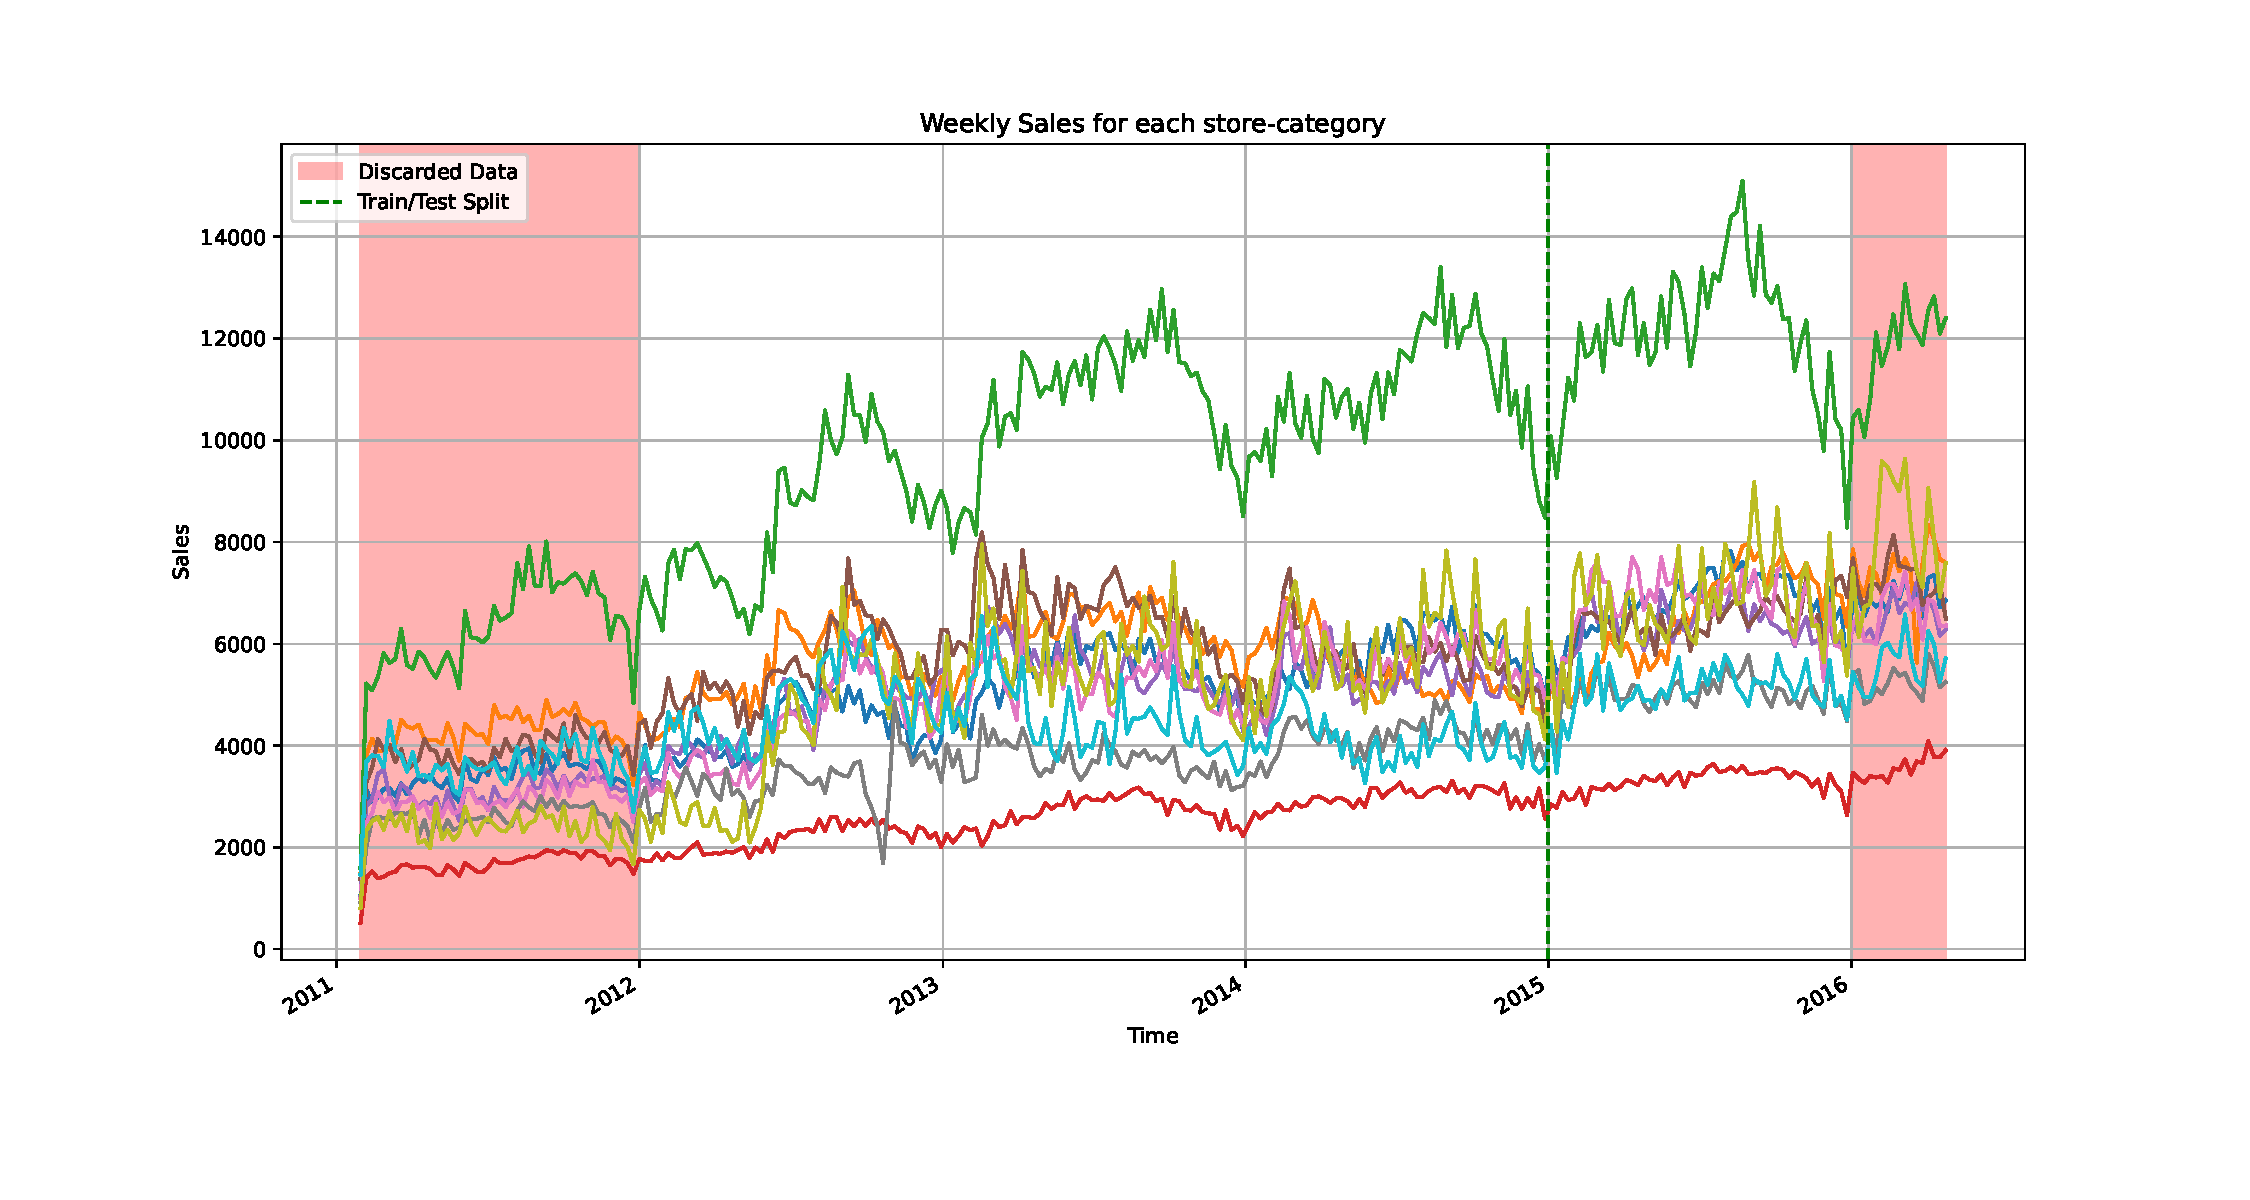
\includegraphics[width=1\textwidth]{./figures/raw_data.pdf}
	\caption{Weekly Sales for Each Store-Category}
	\label{fig:weekly_sales}
\end{figure}


\section{Metric}
In order to quantify and compare the accuracy of different forecasting algorithms, the Mean Absolute Scaled Error (MASE)
\begin{equation}
	\text{MASE} = \frac{\text{mean absolute forecasting error}}{\text{mean gradient in training data}}
\end{equation}
is used. The mean gradient in the training data represents the average forecasting error when using the Naive forecast (predict the next timestep to be equal to the current), and so the MASE represent how good a model is relative to this. This study will consider simultaneous forecasting of ten time series ($N_{\text{time series}} = 10$) (see figure \ref{fig:weekly_sales}) over a forecast horizon of $26$ weeks ($N_{\text{forecast horizon}} = 26$) and so a bit of notation must be introduced to handle this. In order to produce a robust estimate of the MASE, an ensemble of $N_{\text{ensemble}}$ forecasts are consider. The ensemble is produced by producing forecasts for each element in on the interval
\begin{equation}
	[N-(N_{\text{ensemble}}+N_{\text{forecast horizon}}),N-N_{\text{forecast horizon}}]
\end{equation}
where $N$ is the number of datapoints in the time series (all have the same number of data points for simplicity). For each time step in the forecast horizon, there will therefore be $N_{\text{ensemble}}$ values from which to determine a MASE for each time series and forecast time step. Let $f_{i,j,q}$ and $y_{i,j,q}$ denote the model forecast and data, respectively, for time step $i$, time series $j$ and ensemble number $q$ then
\begin{equation}
	\text{MASE}_{i,j} = \frac{\frac{1}{N_{\text{ensemble}}}\sum_{q = 1}^{N_{\text{ensemble}}}|f_{i,j,q}-y_{i,j,q}|}{\frac{1}{N_{\text{training}}-1}\sum_{i = 1}^{N_{\text{training}}}|y_{i-2,j}-y_{i,j}|}
	\label{eq:MASe}
\end{equation}
where $N_{\text{training}}\equiv N-(N_{\text{ensemble}}+N_{\text{forecast horizon}})-1$ represent the part of the data that is common to all ensembles. To condense the information, the MASE can be averaged over time series
\begin{equation}
	\text{MASE}_i \equiv \frac{1}{N_{\text{time series}}}\sum_{j=1}^{N_{\text{time series}}} \text{MASE}_{i,j}
	\label{eq:MASE_avg_series}
\end{equation}
where
\begin{equation}
	\text{MASE}_i \equiv \text{Average MASE over time series}
\end{equation}
and again over the forecast horizon
\begin{equation}
	\braket{\text{MASE}}\equiv \frac{1}{N_{\text{forecast horizon}}N_{\text{time series}}}\sum_{i=1}^{N_{\text{forecast horizon}}}\sum_{j=1}^{N_{\text{time series}}} \text{MASE}_{i,j}
\end{equation}
where for shorthand
\begin{equation}
	\braket{\text{MASE}} \equiv \text{Average MASE over time series and forecast horizon}.
	\label{eq:MASE_avg}
\end{equation}
As a \emph{rough} estimate of uncertainty for equation \eqref{eq:MASE_avg}, the standard deviation of the average over time series is considered
\begin{equation}
	\delta\braket{\text{MASE}} = \sqrt{\frac{1}{N_{\text{forecast horizon}}-1} \sum_{i=1}^{N_{\text{forecast horizon}}} (\text{MASE}_i - \braket{\text{MASE}})^2}
\end{equation}
which assumes the variation between time series can be neglected relative to the variation due between forecast horizon steps. The uncertainty is intended to be a conservative estimate of the variance in the sample rather than the uncertainty of the mean estimate (if the latter is intended, the variance in equation \eqref{eq:MASE_avg_series} and error propagation can be used). Equation \eqref{eq:MASE_avg_series} and \eqref{eq:MASE_avg} are shown for the models considered in figure \ref{fig:avg_mase_over_time_series} and \ref{fig:avg_mase_over_time_series_and_forecast_horizon}, respectively.